\documentclass[11pt]{beamer}

\usetheme{metropolis}


\usepackage[utf8]{inputenc}
\usepackage{ucs}
\usepackage[brazil]{babel}
\usepackage[T1]{fontenc}
\usepackage{amsmath}
\usepackage{amsfonts}
\usepackage{amssymb}
\usepackage{graphicx}
\usepackage{subfigure}
\usepackage{ragged2e}
\usepackage{fancybox}
\usepackage{tikz}



\usepackage{color}
\usepackage{fancyhdr}
\pagestyle{fancy}
\usepackage{xcolor}
\usepackage{xwatermark}

\title{CAPITULO 3 \\ Distribuição geométrica}
\author{Márcia}
\institute{Instituto de Matemática e Estatística \\Faculdade de Estatística}
\date{2019}





\begin{document}

\maketitle
%%%%%%%%%%%%%%%%%%%%%%%%%%%%%%%%%%%%

\section{Distribuição geométrica}

%%%%%%%%%%%%%%%%%%%%%%%%%%%%%%%%%%%%

\subsection{Distribuição Bernoulli}

\begin{frame}
\frametitle{Experimento de Milgram}

\twocol{0.6}{0.4}{

\begin{itemize}

\item Stanley Milgram, psicólogo da Universidade de Yale, conduziu uma série de experimentos sobre obediência à autoridade a partir de 1963.

\item Experimentador (E) ordena que o professor (T), o sujeito do experimento, dê severos choques elétricos a um aluno (L) toda vez que o aluno responder a uma pergunta incorretamente.

\item O aluno é na verdade um ator, e os choques elétricos não são reais, mas um som pré-gravado é tocado toda vez que o professor administra um choque elétrico.

\end{itemize}

}
{
\begin{center}
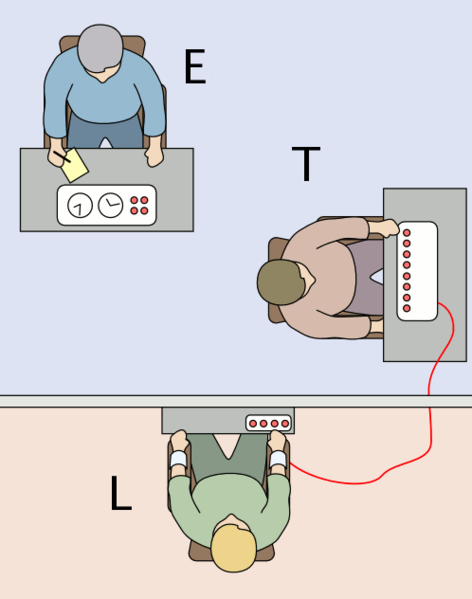
\includegraphics[width=\textwidth]{milgram.png}
\end{center}
\ct{\webURL{http://en.wikipedia.org/wiki/File:Milgram_Experiment_v2.png}}
}

\end{frame}

%%%%%%%%%%%%%%%%%%%%%%%%%%%%%%%%%%%%

\begin{frame}
\frametitle{Experimento de Milgram (cont.)}

\begin{itemize}

\item Esses experimentos mediram a disposição dos participantes do estudo em obedecer a uma figura de autoridade que os instruiu a realizar atos que conflitassem com sua consciência pessoal.

\item Milgram descobriu que cerca de 65 \% das pessoas obedeceriam à autoridade e dariam tais choques.

\item Ao longo dos anos, pesquisas adicionais sugeriram que esse número é aproximadamente consistente entre as comunidades e o tempo.

\end{itemize}

\end{frame}


%%%%%%%%%%%%%%%%%%%%%%%%%%%%%%%%%%%%

\begin{frame}
\frametitle{Variáveis aleatórias de Bernoulli}

\begin{itemize}

\item Cada pessoa na experiência de Milgram pode ser pensada como uma \hl{tentativas}.

\item Uma pessoa é rotulada como \hl{sucesso} se ela se recusar a administrar um choque grave e \hl{falha} se ela administrar tal choque.

\item Como apenas 35 \% das pessoas se recusaram a administrar um choque, \hl{probabilidade de sucesso} é \mathhl{p = 0.35}.

\item Quando uma tentativa individual tem apenas dois resultados possíveis, ela é chamada de \hl{variável aleatória de Bernoulli}.

\end{itemize}

\end{frame}

%%%%%%%%%%%%%%%%%%%%%%%%%%%%%%%%%%%%

\subsection{Distribuição geométrica}

\begin{frame}
\frametitle{Distribuição geométrica}

{\small

\dq{O Dr. Smith quer repetir os experimentos de Milgram, mas ela só quer provar as pessoas até encontrar alguém que não cause um choque severo. Qual é a probabilidade de ela parar depois da primeira pessoa?}

\[ P(1^{0}~pessoa~recusa) = 0.35 \]

\pause

\dq{... a terceira pessoa?}
\[ P(1^{0}~e~2^{0}~choque,~3^{0}~recusa) = \slot{S}{0.65} \times \slot{S}{0.65} \times  \slot{R}{0.35} = 0.65^2 \times 0.35 \approx 0.15 \]

\pause

\dq{... a décima pessoa?}
\soln{
\pause
\[ P(9~choque,~10^{0}~recusa) = \underbrace{\slot{S}{0.65} \times \cdots \times \slot{S}{0.65}}_{9~deste} \times  \slot{R}{0.35} = 0.65^9 \times 0.35 \approx 0.0072 \]
}
}

\end{frame}

%%%%%%%%%%%%%%%%%%%%%%%%%%%%%%%%%%%%

\begin{frame}
\frametitle{Distribuição geométrica (cont.)}

\hl{Distribuição geométrica} descreve o tempo de espera até um sucesso para variáveis aleatórias \hl{independentes e identicamente distribuídas (iid)} Bernoulli.
\begin{itemize}
\item independência: os resultados dos ensaios não afetam uns aos outros
\item idêntico: a probabilidade de sucesso é a mesma para cada tentativa
\end{itemize}

$\:$ \\
$\:$ \\

\pause

\formula{Probabilidades geométricas}{Se $ p $ representar probabilidade de sucesso, $ (1-p) $ representa probabilidade de falha e $ n $ representa número de tentativas independentes \[P(sucesso~na~n^{0}~tentativa) = (1-p)^{n-1} p\]}

\end{frame}

%%%%%%%%%%%%%%%%%%%%%%%%%%%%%%%%%%%%

\begin{frame}

\pq{Podemos calcular a probabilidade de sair um 6 pela primeira vez na 6 $ ^ {0} $ jogada de um dado usando a distribuição geométrica? Note que o que foi um sucesso (sair um 6) e o que foi um fracasso (não sair um 6) estão claramente definidos e um ou outro deve acontecer para cada tentativa.}

\begin{enumerate}[(a)]
\item não, no lançamento de um dado há mais de dois resultados possíveis
\only<1>{\item sim, porque não}
\soln{\only<2>{\item \orange{sim, porque não}}}
\end{enumerate}

\soln{
\only<2>{
\[P(6~na~6^{0}~jogada) = \pr{ \frac{5}{6} }^5 \pr{ \frac{1}{6} } \approx 0.067 \]
}
}

\end{frame}

%%%%%%%%%%%%%%%%%%%%%%%%%%%%%%%%%%%%

\begin{frame}
\frametitle{Valor esperado}

\dq{Quantas pessoas o Dr. Smith espera testar antes de encontrar o primeiro que se recusa a administrar o choque?}

\pause

O valor esperado, ou a média, de uma distribuição geométrica é definida como $\frac{1}{p}$.
\[ \mu = \frac{1}{p} = \frac{1}{0.35} = 2.86 \]

\pause

Ela deve testar 2,86 pessoas antes de encontrar o primeiro que se recusa a administrar o choque.

\pause

Mas como ela pode testar um número decimal de pessoas?

\end{frame}

%%%%%%%%%%%%%%%%%%%%%%%%%%%%%%%%%%%%

\begin{frame}
\frametitle{Valor esperado e sua variabilidade}

\formula{Média e desvio padrão da distribuição geométrica}{
\[ \mu = \frac{1}{p} \qquad \qquad \sigma = \sqrt{\frac{1-p}{p^2}} \] 
}

\pause

\begin{itemize}

\item Voltando à experiência do Dr. Smith:

\[ \sigma = \sqrt{\frac{1-p}{p^2}} = \sqrt{\frac{1-0.35}{0.35^2}} = 2.3 \]

\pause

\item Espera-se que o Dr. Smith teste 2,86 pessoas antes de encontrar o primeiro que se recusa a administrar o choque, mais ou menos 2,3 pessoas.

\pause

\item Esses valores só fazem sentido no contexto de repetir o experimento muitas vezes.

\end{itemize}

\end{frame}

%%%%%%%%%%%%%%%%%%%%%%%%%%%%%%%%%%%%



\end{document}
